\chapter{Sensitivity Analysis}
\begin{outcome}
\begin{itemize}
\item Understand what happens to the optimal solution as we slightly vary the parameters
\item Calculate the range of parameters where the optimal solution (or optimal basis) remains optimal.
\item Understand the change of objective function value as parameters are changed.
\end{itemize}
\end{outcome}


Sensitivity analysis examines how changes in the parameters (objective function coefficients, constraint right-hand sides) affect the optimal solution. This can be computed from the final simplex dictionary, often provided by optimization software such as Excel Solver.

We begin this section with an interactive desmos example.  Go to \href{https://www.desmos.com/calculator/xz1f0tdjf9}{Desmos LP Sensitivity!}.



\subsection{Mathematical details of sensitivity analysis}

We now analyze how changes in different parameters affect the optimal solution.

\subsection{Effect of Changing an Objective Coefficient \( c_i \)}

\textbf{How it appears in the dictionary:}  
The objective function in the revised dictionary is:
\[
z = \mathbf{c}_B^\top A_B^{-1} \mathbf{b} + (\mathbf{c}_N^\top - \mathbf{c}_B^\top A_B^{-1} A_N) \mathbf{x}_N.
\]
The coefficients of \( \mathbf{x}_N \) are known as the \textbf{reduced costs}:
\[
\mathbf{c}_N^\top - \mathbf{c}_B^\top A_B^{-1} A_N.
\]

\textbf{Analysis:}
\begin{itemize}
    \item If \( i \) is a \textbf{basic variable}, \( c_i \) appears in \( \mathbf{c}_B \), and since \( z^* \) contains \( \mathbf{c}_B^\top A_B^{-1} \mathbf{b} \), a change in \( c_i \) directly affects the optimal objective function in a linear manner.
    \item If \( i \) is a \textbf{non-basic variable}, \( c_i \) appears in \( \mathbf{c}_N \). The optimal basis remains unchanged, so the optimal objective function does \textbf{not} change. However, if the reduced cost \( (\mathbf{c}_N^\top - \mathbf{c}_B^\top A_B^{-1} A_N) \) changes sign, the variable may enter the basis.
\end{itemize}

\textbf{Key Takeaways:}
\begin{itemize}
    \item Changing the coefficient of a \textbf{basic variable} shifts the objective function \textbf{linearly}.
    \item Changing the coefficient of a \textbf{non-basic variable} does not affect the objective value \textbf{unless it becomes negative}, triggering a basis change.
\end{itemize}

\subsection{Effect of Changing the Right-Hand Side \( \mathbf{b} \)}

\textbf{How it appears in the dictionary:}  
The basic solution is:
\[
\mathbf{x}_B = A_B^{-1} \mathbf{b}.
\]

\textbf{Analysis:}
\begin{itemize}
    \item \textbf{Direct effect on feasibility:} Since \( \mathbf{x}_B \geq 0 \) is a feasibility condition, changes in \( \mathbf{b} \) directly affect feasibility.
    \item \textbf{Basis stability:}
    \begin{itemize}
        \item If \( \mathbf{b} \) changes slightly, the basis may remain optimal, but \( \mathbf{x}_B \) is rescaled accordingly.
        \item If \( \mathbf{b} \) changes significantly, one or more basic variables may become \textbf{negative}, requiring a pivot to restore feasibility.
    \end{itemize}
    \item \textbf{Impact on objective function:}
    \begin{itemize}
        \item Since \( z^* = \mathbf{c}_B^\top A_B^{-1} \mathbf{b} \), the objective value scales with \( \mathbf{b} \).
        \item Small changes in \( \mathbf{b} \) result in proportional changes in \( z^* \), assuming the basis remains optimal.
    \end{itemize}
\end{itemize}

\textbf{Key Takeaways:}
\begin{itemize}
    \item Changing \( \mathbf{b} \) \textbf{directly modifies} the basic solution.
    \item Large changes can force a \textbf{basis change} or make the problem \textbf{infeasible}.
    \item The \textbf{objective value scales} with \( \mathbf{b} \).
\end{itemize}

\subsection{Effect of Changing the Coefficients \( a_{ij} \) of the Constraint Matrix \( A \)}

\textbf{How it appears in the dictionary:}  
The basic variables satisfy:
\[
\mathbf{x}_B = A_B^{-1} \mathbf{b}.
\]

If \( A \) changes, then \( A_B^{-1} \) changes, which affects:
\begin{enumerate}
    \item \textbf{The basic solution \( \mathbf{x}_B \).}
    \item \textbf{The reduced costs \( \mathbf{c}_N^\top - \mathbf{c}_B^\top A_B^{-1} A_N \)} in the objective function.
\end{enumerate}

\textbf{Analysis:}
\begin{itemize}
    \item \textbf{Geometric Interpretation:} Changing \( a_{ij} \) \textbf{tilts} the corresponding constraint, altering the feasible region.
    \item \textbf{If \( i \) is a non-basic variable:}
    \begin{itemize}
        \item The structure of \( A_B^{-1} \) remains unchanged.
        \item The optimal basis remains unchanged.
        \item The optimal solution \textbf{does not change}.
    \end{itemize}
    \item \textbf{If \( i \) is a basic variable:}
    \begin{itemize}
        \item Since \( A_B^{-1} \) depends on the inverse of the basis matrix, \textbf{even small changes in \( A_B \) can have large effects}.
        \item The optimal solution and reduced costs change, potentially leading to a basis change.
    \end{itemize}
\end{itemize}

\textbf{Key Takeaways:}
\begin{itemize}
    \item If \( a_{ij} \) belongs to a \textbf{non-basic variable}, the optimal solution \textbf{remains unchanged}.
    \item If \( a_{ij} \) belongs to a \textbf{basic variable}, it \textbf{modifies \( A_B^{-1} \)}, causing significant changes to the optimal solution.
    \item The constraints are \textbf{tilted}, altering the feasible region.
\end{itemize}

\subsection{Summary Table: Sensitivity Effects in the Revised Simplex Dictionary}

\[
\begin{array}{|c|c|c|c|}
\hline
\textbf{Change Type} & \textbf{Effect on Basic Solution} & \textbf{Effect on Objective} & \textbf{Basis Change?} \\
\hline
c_i \text{ (objective coefficient)} & \text{Only if \( i \) is in basis} & \text{Yes, if \( i \) is basic} & \text{If reduced cost changes sign} \\
\hline
\mathbf{b} \text{ (RHS vector)} & \text{Always changes} & \text{Always scales} & \text{If infeasibility occurs} \\
\hline
a_{ij} \text{ (constraint matrix)} & \text{Only if \( i \) is in basis} & \text{Changes reduced costs} & \text{If basis becomes infeasible} \\
\hline
\end{array}
\]

\subsection{Computing the Range of Parameters That Maintain the Optimal Basis}

In this section, we analyze the sensitivity of the optimal basis to changes in different problem parameters. Specifically, we examine:
\begin{enumerate}
    \item Changes in the right-hand side (RHS) value of the first constraint.
    \item Changes in one of the objective function coefficients.
\end{enumerate}
We determine the range of values these parameters can take while preserving the current optimal basis.


Note that we could also have written this as 
\[
\begin{aligned}
\text{Maximize} \quad & \mathbf{c}^\top \mathbf{x} \\
\text{subject to} \quad & A_x\mathbf{x} + I\mathbf{s}  = \mathbf{b}, \\
& \mathbf{x}, \mathbf{s} \geq \mathbf{0}
\end{aligned}
\]
where 
\[
A_x =
\begin{bmatrix}
1 & 1 \\
2 & 1 \\
1 & 2 
\end{bmatrix},
\text{ and }
\mathbf{x} = 
\begin{bmatrix}
x \\
y \\
\end{bmatrix},
\mathbf{s} = 
\begin{bmatrix}
s_1 \\
s_2 \\
s_3
\end{bmatrix}\]



\section{Sensitivity Analysis: Right-Hand Side Perturbations}

After applying the simplex method, we obtain the following optimal dictionary:

\begin{tcolorbox}[colback=green!5!white, colframe=green!75!black,    
    width=1\textwidth,
    box align=center, 
    title=\textbf{Final Dictionary}]
\[
\begin{aligned}
\text{Maximize} \quad 
& z = 23 - s_1 - s_3 \\
\text{subject to} \quad 
& x = 4 - 2s_1 + s_3, \\
& y = 5 + s_1 - s_3, \\
& s_2 = 3 + 3s_1 - s_3, \\
& x, y, s_1, s_2, s_3 \geq 0.
\end{aligned}
\]
The current basis is \( B = \{x, y, s_2\} \), with nonbasic variables \( N = \{s_1, s_3\} \).

The optimal solution is:
\[
(x, y, s_2, s_1, s_3) = (4, 5, 3, 0, 0) \quad \text{with} \quad z = 23.
\]
\end{tcolorbox}

\subsection*{Goal: Understanding Sensitivity to RHS Changes}

In standard form, a linear program is written as \( A\mathbf{x} = \mathbf{b}, \ \mathbf{x} \geq 0 \). Sensitivity analysis explores how the optimal solution and objective value change when we perturb entries of \( \mathbf{b} \), while holding the objective coefficients and constraint matrix fixed.

\bigskip

In particular, we want to answer:
\begin{enumerate}
    \item For which changes in the RHS does the current basis remain optimal?
    \item How does the optimal solution vary with these changes?
    \item How does the objective value change?
\end{enumerate}

We consider changes to each component of the RHS independently, starting with the second constraint.

\subsection{Perturbing \( b_2 \): A Basic Slack Variable}

The second constraint (corresponding to slack variable \( s_2 \)) originally has RHS value \( b_2 = 16 \). We now perturb this to \( 16 + \Delta \), where \( \Delta \in \mathbb{R} \), and investigate the effect.

\begin{tcolorbox}[colback=gray!5!white, colframe=pink!75!black,    
    width=0.9\textwidth,
    box align=center, 
    title=\textbf{Perturbed Standard Form (RHS of Constraint 2)}]
\[
\begin{aligned}
\text{Maximize} \quad & 2x + 3y \\
\text{subject to} \quad 
& x + y + s_1 = 9 \quad & \text{(hours)} \\
& 2x + y + s_2 = 16 + \Delta \quad & \text{(flour)} \\
& x + 2y + s_3 = 14 \quad & \text{(sugar)} \\
& x, y, s_1, s_2, s_3 \geq 0
\end{aligned}
\]

To isolate the effect of \( \Delta \), define a new variable:
\[
s_2:= s_2' + \Delta \quad \Rightarrow \quad s_2' = s_2 - \Delta.
\]

Substituting into the system yields:
\[
\begin{aligned}
\text{Maximize} \quad & 2x + 3y \\
\text{subject to} \quad 
& x + y + s_1 = 9 \\
& 2x + y + s_2= 16 + \Delta  & \Rightarrow &&  2x + y + s_2'= 16\\
& x + 2y + s_3 = 14 \\
& x, y, s_1, s_2', s_3 \geq 0
\end{aligned}
\]
\end{tcolorbox}

\subsubsection*{Adapting the Final Dictionary}

Since the structure of the problem remains the same in terms of the new variable \( s_2' \), we can substitute into the final dictionary:

\[
\begin{aligned}
\text{Maximize} \quad 
& z = 23 - s_1 - s_3 \\
\text{subject to} \quad 
& x = 4 - 2s_1 + s_3 \\
& y = 5 + s_1 - s_3 \\
& s_2'  = 3 + 3s_1 - s_3 
\quad \Rightarrow \quad
s_2 - \Delta = 3  + 3s_1 - s_3 \\
& x, y, s_1, s_2', s_3 \geq 0
\end{aligned}
\]

To remain optimal, the dictionary must still satisfy feasibility: all basic variables must remain nonnegative when \( s_1 = s_3 = 0 \). So:

\[
s_2' = 3 + \Delta \geq 0 \quad \Longleftrightarrow \quad \boxed{\Delta \geq -3}.
\]
Equivalently, since \( b_2 = 16 + \Delta \), we require:
\[
\boxed{b_2 \geq 13}.
\]


\subsection*{Conclusion}

The current basis \( B = \{x, y, s_2\} \) remains optimal under the RHS perturbation \( b_2 = 16 + \Delta \) as long as:
\[
\boxed{\Delta \geq -3} \Rightarrow b_2 \geq 13
\]

Beyond this range, \( s_2 < 0 \), and the current dictionary becomes infeasible — triggering a new pivot in the simplex method.


\subsection{Perturbing \( b_1 \): A Nonbasic Slack Variable}

The first constraint corresponds to slack variable \( s_1 \), which is currently \emph{nonbasic} and set to 0 in the optimal solution. Its original right-hand side is \( b_1 = 9 \). We now perturb it to \( 9 + \Delta \), where \( \Delta \in \mathbb{R} \), and examine how this affects the dictionary.

\begin{tcolorbox}[colback=gray!5!white, colframe=pink!75!black,    
    width=0.9\textwidth,
    box align=center, 
    title=\textbf{Perturbed Standard Form (RHS of Constraint 1)}]
\[
\begin{aligned}
\text{Maximize} \quad & 2x + 3y \\
\text{subject to} \quad 
& x + y + s_1 = 9 + \Delta \quad & \text{(hours)} \\
& 2x + y + s_2 = 16 \quad & \text{(flour)} \\
& x + 2y + s_3 = 14 \quad & \text{(sugar)} \\
& x, y, s_1, s_2, s_3 \geq 0
\end{aligned}
\]

To isolate the effect of \( \Delta \), define a new variable:
\[
s_1 := s_1' - \Delta \quad \Rightarrow \quad s_1' = s_1 + \Delta.
\]

Substituting into the system yields:
\[
\begin{aligned}
x + y + s_1 &= 9 + \Delta \\
x + y + (s_1' - \Delta) &= 9 + \Delta \\
x + y + s_1' &= 9
\end{aligned}
\]
So the perturbed system is equivalent to the original, but now expressed in terms of \( s_1' \).
\end{tcolorbox}

\subsubsection*{Updated Dictionary}

We substitute \( s_1 = s_1' - \Delta \) into the optimal dictionary:

\[
\begin{aligned}
\text{Maximize} \quad 
z &= 23 - s_1 - s_3 = 23 - (s_1' - \Delta) - s_3 = (23 + \Delta) - s_1' - s_3 \\
x &= 4 - 2s_1 + s_3 = 4 - 2(s_1' - \Delta) + s_3 = (4 + 2\Delta) - 2s_1' + s_3 \\
y &= 5 + s_1 - s_3 = 5 + (s_1' - \Delta) - s_3 = (5 - \Delta) + s_1' - s_3 \\
s_2 &= 3 + 3s_1 - s_3 = 3 + 3(s_1' - \Delta) - s_3 = (3 - 3\Delta) + 3s_1' - s_3
\end{aligned}
\]

To ensure the basis remains feasible, set \( s_1' = s_3 = 0 \) and check that the basic variables remain nonnegative:
\[
x = 4 + 2\Delta, \quad
y = 5 - \Delta, \quad
s_2 = 3 - 3\Delta
\]

Feasibility conditions:
\[
\begin{aligned}
x \geq 0 &\Rightarrow \Delta \geq -2 \\
y \geq 0 &\Rightarrow \Delta \leq 5 \\
s_2 \geq 0 &\Rightarrow \Delta \leq 1
\end{aligned}
\]

Thus, all conditions are satisfied when:
\[
\boxed{-2 \leq \Delta \leq 1}
\]

\subsubsection*{Conclusions}
\begin{itemize}
\item The current basis \( B = \{x, y, s_2\} \) remains optimal under the perturbation \( b_1 = 9 + \Delta \) as long as:
\[
\boxed{-2 \leq \Delta \leq 1} \quad \Rightarrow \quad \boxed{7 \leq b_1 \leq 10}
\]
\item Within this range, the objective value changes linearly as:
\[
z = 23 + \Delta.
\]
\item Outside this range, one or more basic variables becomes negative, and the current solution becomes infeasible, prompting a new pivot in the simplex method.
\end{itemize}


\subsection{Perturbing \( b_3 \): Another Nonbasic Slack Variable}

The third constraint corresponds to slack variable \( s_3 \), which is currently \emph{nonbasic} and equal to 0 in the optimal solution. Its original right-hand side is \( b_3 = 14 \). We now perturb it to \( 14 + \Delta \), where \( \Delta \in \mathbb{R} \), and examine how this affects the dictionary.

\begin{tcolorbox}[colback=gray!5!white, colframe=pink!75!black,    
    width=0.9\textwidth,
    box align=center, 
    title=\textbf{Perturbed Standard Form (RHS of Constraint 3)}]
\[
\begin{aligned}
\text{Maximize} \quad & 2x + 3y \\
\text{subject to} \quad 
& x + y + s_1 = 9 \quad & \text{(hours)} \\
& 2x + y + s_2 = 16 \quad & \text{(flour)} \\
& x + 2y + s_3 = 14 + \Delta \quad & \text{(sugar)} \\
& x, y, s_1, s_2, s_3 \geq 0
\end{aligned}
\]

To isolate the effect of \( \Delta \), define a new variable:
\[
s_3 := s_3' - \Delta \quad \Rightarrow \quad s_3' = s_3 + \Delta.
\]

Substituting into the system yields:
\[
x + 2y + (s_3' - \Delta) = 14 + \Delta \quad \Rightarrow \quad x + 2y + s_3' = 14.
\]
So the perturbed system returns to the original structure but in terms of \( s_3' \).
\end{tcolorbox}

\subsubsection*{Updated Dictionary}

Substitute \( s_3 = s_3' - \Delta \) into the optimal dictionary:

\[
\begin{aligned}
\text{Maximize} \quad 
z &= 23 - s_1 - s_3 = 23 - s_1 - (s_3' - \Delta) = (23 + \Delta) - s_1 - s_3' \\
x &= 4 - 2s_1 + s_3 = 4 - 2s_1 + (s_3' - \Delta) = (4 - \Delta) - 2s_1 + s_3' \\
y &= 5 + s_1 - s_3 = 5 + s_1 - (s_3' - \Delta) = (5 + \Delta) + s_1 - s_3' \\
s_2 &= 3 + 3s_1 - s_3 = 3 + 3s_1 - (s_3' - \Delta) = (3 + \Delta) + 3s_1 - s_3'
\end{aligned}
\]

Now test feasibility at the basic solution \( s_1 = s_3' = 0 \):

\[
x = 4 - \Delta, \quad
y = 5 + \Delta, \quad
s_2 = 3 + \Delta
\]

Feasibility requires:
\[
\begin{aligned}
x \geq 0 &\Rightarrow \Delta \leq 4 \\
s_2 \geq 0 &\Rightarrow \Delta \geq -3
\end{aligned}
\]

Thus, the allowable range for \( \Delta \) is:
\[
\boxed{-3 \leq \Delta \leq 4}
\]

\subsubsection*{Conclusion}

\begin{itemize}
\item The current basis \( B = \{x, y, s_2\} \) remains optimal under the perturbation \( b_3 = 14 + \Delta \) as long as:
\[
\boxed{-3 \leq \Delta \leq 4} \quad \Rightarrow \quad \boxed{11 \leq b_3 \leq 18}
\]
\item Within this range, the objective value changes linearly as:
\[
z = 23 + \Delta.
\]
\item Outside this range, \( x < 0 \) or \( s_2 < 0 \), and the dictionary becomes infeasible.
\end{itemize}



\subsection{Perturbing \( c_1 \) and \( c_2 \): Objective Coefficients of Basic Variables}

We now examine how changes to the objective function coefficients affect the optimality of the current basis. In the original problem, the objective is:
\[
\text{Maximize} \quad 2x + 3y.
\]
We now perturb these coefficients to:
\[
\text{Maximize} \quad (2 + \delta_1)x + (3 + \delta_2)y,
\]
where \( \delta_1, \delta_2 \in \mathbb{R} \).

From the final dictionary, we have:
\[
\begin{aligned}
z &= 23 - s_1 - s_3 \\
x &= 4 - 2s_1 + s_3 \\
y &= 5 + s_1 - s_3 \\
s_2 &= 3 + 3s_1 - s_3,
\end{aligned}
\]
with basis \( B = \{x, y, s_2\} \) and nonbasic variables \( N = \{s_1, s_3\} \).

\subsubsection*{Perturbing \( c_1 \): Objective Coefficient of \( x \)}

Let \( c_1 = 2 + \delta_1 \). Since \( x \) is basic, the perturbed objective becomes:
\[
z = 23 + \delta_1 \cdot x = 23 + \delta_1(4 - 2s_1 + s_3)
= (23 + 4\delta_1) + (-2\delta_1)s_1 + \delta_1 s_3.
\]

Adding to the original dictionary \( z = 23 - s_1 - s_3 \), we obtain:
\[
z = (23 + 4\delta_1) + (-1 - 2\delta_1)s_1 + (-1 + \delta_1)s_3.
\]

To maintain optimality, the reduced costs of nonbasic variables \( s_1 \) and \( s_3 \) must remain \( \leq 0 \). Thus:
\[
\begin{aligned}
-1 - 2\delta_1 &\leq 0 \quad \Rightarrow \quad \delta_1 \geq -\tfrac{1}{2}, \\
-1 + \delta_1 &\leq 0 \quad \Rightarrow \quad \delta_1 \leq 1.
\end{aligned}
\]

So the allowable range for \( \delta_1 \) is:
\[
\boxed{-\tfrac{1}{2} \leq \delta_1 \leq 1} \quad \Rightarrow \quad \boxed{1.5 \leq c_1 \leq 3}.
\]

Within this range, the objective value changes linearly as:
\[
z = 23 + 4\delta_1.
\]

\subsubsection*{Perturbing \( c_2 \): Objective Coefficient of \( y \)}

Let \( c_2 = 3 + \delta_2 \). Since \( y \) is also basic, the perturbed objective becomes:
\[
z = 23 + \delta_2 \cdot y = 23 + \delta_2(5 + s_1 - s_3)
= (23 + 5\delta_2) + \delta_2 s_1 - \delta_2 s_3.
\]

Adding to the original dictionary \( z = 23 - s_1 - s_3 \), we obtain:
\[
z = (23 + 5\delta_2) + (-1 + \delta_2)s_1 + (-1 - \delta_2)s_3.
\]

To maintain optimality:
\[
\begin{aligned}
-1 + \delta_2 &\leq 0 \quad \Rightarrow \quad \delta_2 \leq 1, \\
-1 - \delta_2 &\leq 0 \quad \Rightarrow \quad \delta_2 \geq -1.
\end{aligned}
\]

So the allowable range for \( \delta_2 \) is:
\[
\boxed{-1 \leq \delta_2 \leq 1} \quad \Rightarrow \quad \boxed{2 \leq c_2 \leq 4}.
\]

Within this range, the objective value changes linearly as:
\[
z = 23 + 5\delta_2.
\]

\subsubsection*{Summary of Sensitivity to Objective Coefficients}

\begin{center}
\begin{tabular}{|c|c|c|}
\hline
\textbf{Perturbed Coefficient} & \textbf{Allowed Range} & \textbf{Effect on Objective} \\
\hline
\( c_1 = 2 + \delta_1 \) & \( \boxed{1.5 \leq c_1 \leq 3} \) & \( z = 23 + 4\delta_1 \) \\
\( c_2 = 3 + \delta_2 \) & \( \boxed{2 \leq c_2 \leq 4} \)   & \( z = 23 + 5\delta_2 \) \\
\hline
\end{tabular}
\end{center}

Outside these ranges, the reduced costs of nonbasic variables become positive, violating optimality. In such cases, the simplex method would require a new pivot.


\section{Sensitivity with Matrix Notation}

\begin{tcolorbox}[colback=green!5!white, colframe=green!75!black,    
    width=1\textwidth, % adjust width as desired
    box align=center, 
    title=\textbf{Final Dictionary in Matrix Notation}]
Let the basic variables be $\mathbf{x}_B = \begin{bmatrix} x \\ y \\ s_2 \end{bmatrix}$,
and the non-basic variables be $\mathbf{x}_N = \begin{bmatrix} s_1 \\ s_3 \end{bmatrix}$.
Then the dictionary can be written as:

$$
\mathbf{x}_B = \mathbf{b}' - A_N' \mathbf{x}_N,
$$

where:

$$
\mathbf{b}' = 
\begin{bmatrix}
4 \\
5 \\
3
\end{bmatrix}, \quad
A_N' = 
\begin{bmatrix}
-2 & 1 \\
1 & -1 \\
3 & -1
\end{bmatrix}.
$$

Thus, explicitly:

$$
\begin{bmatrix}
x \\
y \\
s_2
\end{bmatrix}
=
\begin{bmatrix}
4 \\
5 \\
3
\end{bmatrix}
-
\begin{bmatrix}
-2 & 1 \\
1 & -1 \\
3 & -1
\end{bmatrix}
\begin{bmatrix}
s_1 \\
s_3
\end{bmatrix}.
$$
or equivalentely
$$
\begin{bmatrix}
x \\
y \\
s_2
\end{bmatrix}
=
\begin{bmatrix}
4 \\
5 \\
3
\end{bmatrix}
+
s_1
\begin{bmatrix}
2  \\
-1  \\
-3 
\end{bmatrix}
 +s_3
\begin{bmatrix}
 -1 \\
 1 \\
 1
\end{bmatrix}.$$
\end{tcolorbox}


The basis matrix is 
$$
A_B = \begin{bmatrix}
1 & 1 & 0\\
2 & 1 & 1\\
1 & 2 & 0
\end{bmatrix}
\quad \text{ and } \quad
A_B^{-1} = \begin{bmatrix}
2 & 0 & -1\\
-1 & 0 & 1\\
-3 & 1 & 1
\end{bmatrix}.
$$


\begin{remark}{Recovering $A_B^{-1}$}{}
\[
A(x, s) =
\begin{bmatrix}
1 & 0 & 2 & 0 & -1 \\
0 & 1 & -1 & 0 & 1 \\
0 & 0 & -3 & 1 & 1
\end{bmatrix}
\begin{bmatrix}
x \\ y \\ s_1 \\ s_2 \\ s_3
\end{bmatrix}
=
\begin{bmatrix}
4 \\ 5 \\ 3
\end{bmatrix}
\]

Partitioning into basic variables \( x = (x, y) \) and slack variables \( s = (s_1, s_2, s_3) \), we write:
\[
A_x x + A_s s = b
\quad \text{where} \quad
A_x =
\begin{bmatrix}
1 & 0 \\
0 & 1 \\
0 & 0
\end{bmatrix}, \quad
A_s =
\begin{bmatrix}
2 & 0 & -1 \\
-1 & 0 & 1 \\
-3 & 1 & 1
\end{bmatrix}, \quad
b =
\begin{bmatrix}
4 \\ 5 \\ 3
\end{bmatrix}
\]

\text{Hence, since the slack columns came from the identity matrix in the original \( A \), we conclude:}
\[
A_s = A_B^{-1}
\]


\end{remark}




\subsubsection{1. Changing the Right-Hand Side \( b_1 \) of the First Constraint}
We modify the right-hand side of the first constraint and analyze its impact on feasibility:
\[
b_1 \quad \Rightarrow \quad \begin{bmatrix} b_1 \\ 16 \\ 14 \end{bmatrix}.
\]
Using the inverse basis matrix \( A_B^{-1} \), the basic solution is updated as:
\[
\mathbf{x}_B = A_B^{-1} \mathbf{b}.
\]
Ensuring that all basic variables remain non-negative, we derive the feasibility conditions:
\[ 
A_B^{-1} \mathbf{b} = A_B^{-1} = \begin{bmatrix}
2 & 0 & -1\\
-1 & 0 & 1\\
-3 & 1 & 1
\end{bmatrix} \begin{bmatrix} b_1\\ 16\\ 14 \end{bmatrix} 
= 
\begin{bmatrix}
2b_1 - 14\\
-b_1 + 14\\
-3b_1 + 30
\end{bmatrix} \geq 
\begin{bmatrix}
0\\
0\\
0
\end{bmatrix} 
\]
Simplifying, we have
\[
\begin{bmatrix}
b_1 \\
14\\
10
\end{bmatrix} \geq 
\begin{bmatrix}
7\\
b_1\\
b_1
\end{bmatrix} 
\]

\[
7 \leq b_1 \leq 10
\]
is the feasible range for \( b_1 \) that preserves the optimal basis.

In the image here, we show changing $b_1$ to the values of $7,9,10$.
\begin{center}
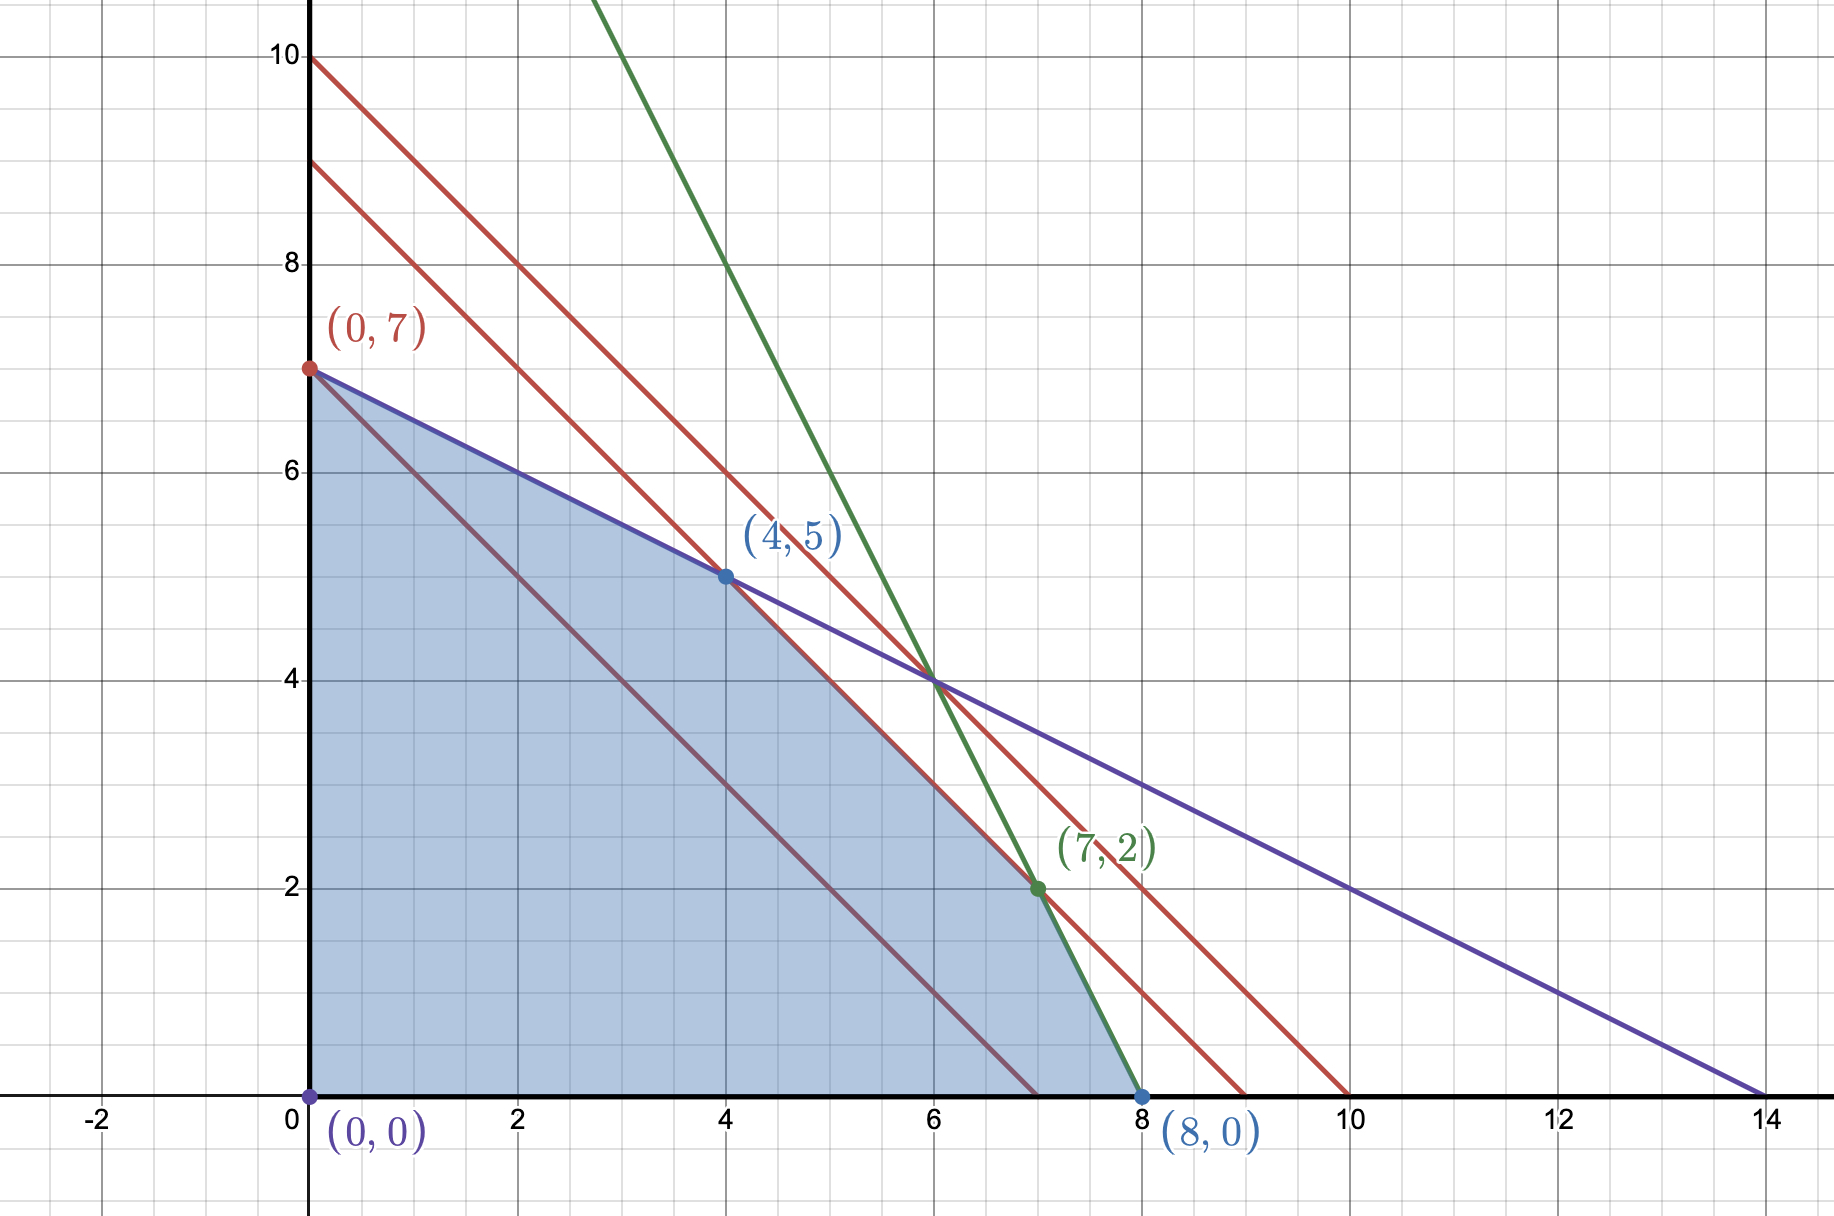
\includegraphics[scale = 0.17]{Figures/sensitivity-changing-b}
\end{center}



\subsubsection{Sensitivity Analysis on the Objective Coefficient \(c_x\)}

To determine the range of values for \( c_x \) (the coefficient of \( x \) in the objective function) such that the current basis remains optimal, we analyze the simplex optimality conditions.

\textbf{Step 1: Compute the Reduced Costs}
The objective function is initially:
\[
    z = 2x + 3y.
\]
The cost vector for all variables is:
\[
    c = \begin{bmatrix} c_x \\ 3 \\ 0 \\ 0 \\ 0 \end{bmatrix}.
\]
The cost vector corresponding to the basic variables \( x, y, s_2 \) (i.e., the basis) is:
\[
    c_B = \begin{bmatrix} c_x & 3 & 0 \end{bmatrix}.
\]
The reduced cost for any non-basic variable \( j \) is given by:
\[
    \bar{c}_j = c_j - c_B A_B^{-1} A_j.
\]
The non-basic variables are \( s_1 \) and \( s_3 \). We need to ensure that their reduced costs remain non-negative.

\textbf{Step 2: Compute the Reduced Costs for \( s_1 \) and \( s_3 \)}
The constraint matrix is:
\[
    A = \begin{bmatrix} 
    1 & 1 & 1 & 0 & 0 \\ 
    2 & 1 & 0 & 1 & 0 \\ 
    1 & 2 & 0 & 0 & 1 
    \end{bmatrix}.
\]
Extracting the columns corresponding to \( s_1 \) and \( s_3 \):
\[
    A_{s_1} = \begin{bmatrix} 1 \\ 0 \\ 0 \end{bmatrix}, \quad
    A_{s_3} = \begin{bmatrix} 0 \\ 0 \\ 1 \end{bmatrix}.
\]
Using the inverse basis matrix:
\[
    A_B^{-1} A_{s_1} = 
    \begin{bmatrix} 
    2 & 0 & -1 \\ 
    -1 & 0 & 1 \\ 
    -3 & 1 & 1
    \end{bmatrix}
    \begin{bmatrix} 1 \\ 0 \\ 0 \end{bmatrix} =
    \begin{bmatrix} 2 \\ -1 \\ -3 \end{bmatrix}.
\]
\[
    A_B^{-1} A_{s_3} = 
    \begin{bmatrix} 
    2 & 0 & -1 \\ 
    -1 & 0 & 1 \\ 
    -3 & 1 & 1
    \end{bmatrix}
    \begin{bmatrix} 0 \\ 0 \\ 1 \end{bmatrix} =
    \begin{bmatrix} -1 \\ 1 \\ 1 \end{bmatrix}.
\]
Thus, the reduced costs are:
\[
    \bar{c}_{s_1} = 0 - \begin{bmatrix} c_x & 3 & 0 \end{bmatrix} \cdot \begin{bmatrix} 2 \\ -1 \\ -3 \end{bmatrix}
    = 0 - (2c_x - 3).
\]
\[
    \bar{c}_{s_3} = 0 - \begin{bmatrix} c_x & 3 & 0 \end{bmatrix} \cdot \begin{bmatrix} -1 \\ 1 \\ 1 \end{bmatrix}
    = 0 - (-c_x + 3).
\]
To retain optimality, we want $\bar{c}_{s_1}$ anr $\bar{c}_{s_3}$ to be $\leq 0$.

\[
    -2c_x + 3 \leq 0 \quad \Rightarrow \quad c_x \geq \frac{3}{2} = 1.5.
\]
\[
    c_x - 3 \leq 0 \quad \Rightarrow \quad c_x \leq 3.
\]

\textbf{Step 3: Feasible Range for \( c_x \)}
For the current basis to remain optimal, \( c_x \) must satisfy:
\[
    1.5 \leq c_x \leq 3.
\]

Thus, we have confirmed that the coefficient \( c_x \) can range between1.5 and 3 while maintaining the current optimal basis.

\begin{center}
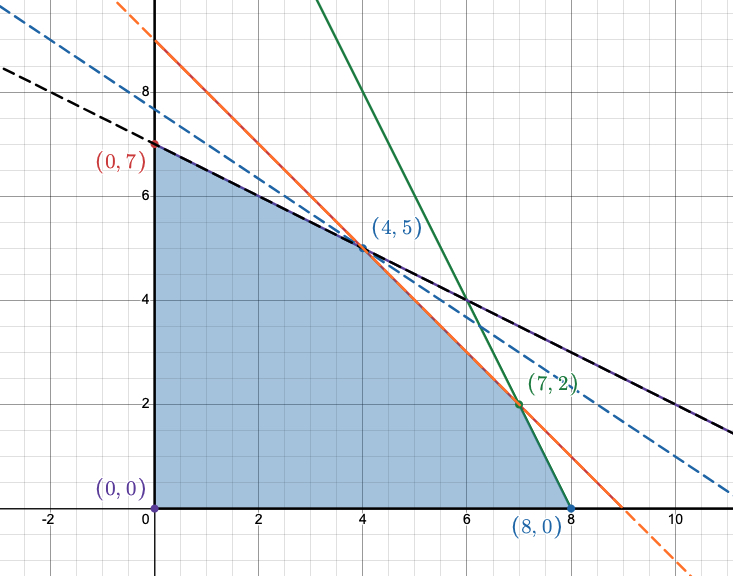
\includegraphics[scale = 0.3]{Figures/sensitivity-objective}
\end{center}


\subsection{Excel Solver Sensitivity Analysis}

When solving a problem in excel, you can ask for a sensitivity analysis.

\begin{center}
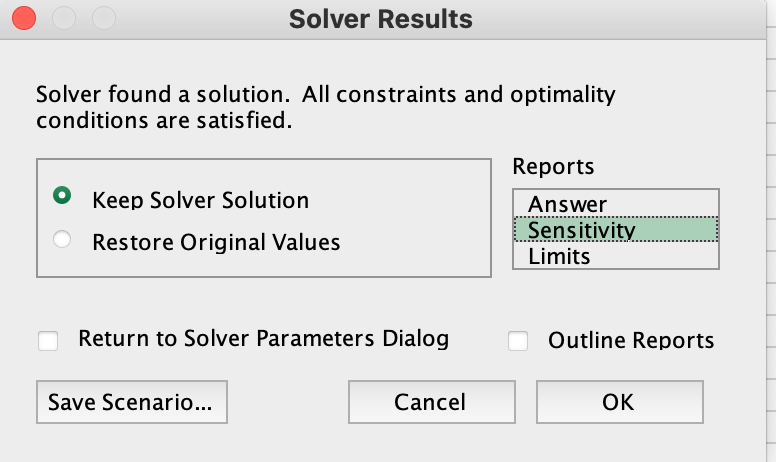
\includegraphics[scale =0.3]{Figures/excel-sensitivity}
\end{center}
This will generate a report that will show the following:
\begin{itemize}
\item \textbf{Allowable Increase/Decrease:} For each decision variable's coefficient in the objective function, the report provides the range (allowable increase and allowable decrease) within which the coefficient can change without altering the current optimal basis. This range indicates the stability of the optimal solution with respect to changes in that coefficient.

\item \textbf{Right-Hand Side (RHS) Values:} For each constraint, the sensitivity report lists the \emph{shadow price} (or dual value), which represents the rate of change in the objective function per unit increase in the RHS of that constraint. It also provides the allowable increase and allowable decrease for the RHS. These values indicate how robust the constraints are; small allowable changes might imply that the solution is sensitive to fluctuations in available resources or demand levels.

\item \textbf{Constraint Status:} The report shows which constraints are binding (active) and which are non-binding. A binding constraint has a positive shadow price and restricts the optimal solution, while a non-binding constraint has a shadow price of zero.
\end{itemize}

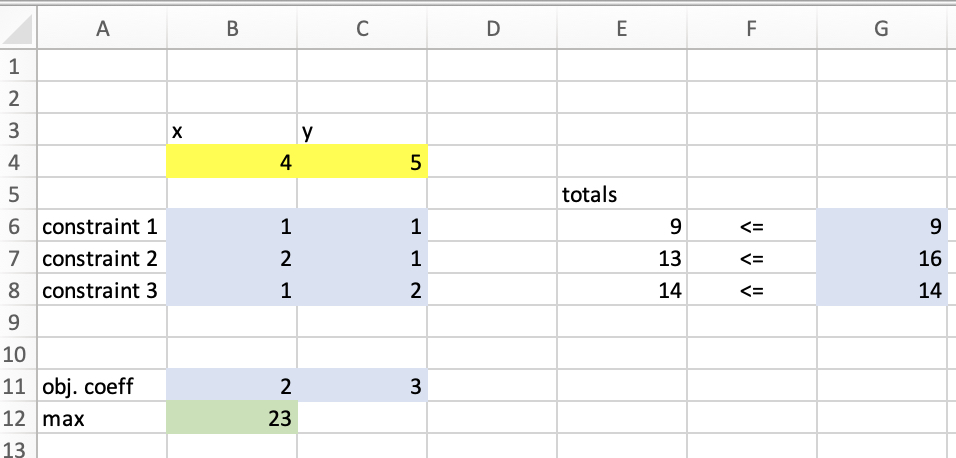
\includegraphics[scale = 0.3]{Figures/excel-setup}
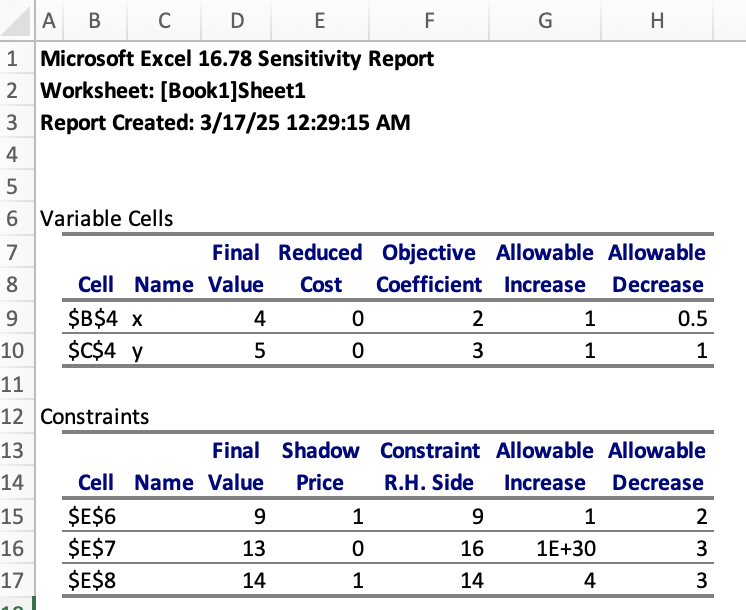
\includegraphics[scale = 0.3]{Figures/excel-sensitivity-report}




